\documentclass[brazil, 12pt]{article}

\usepackage[portuguese]{babel}
\usepackage[utf8]{inputenc}
\usepackage[T1]{fontenc}
\usepackage[dvips]{graphicx}
\usepackage{indentfirst}
\usepackage{caption}
\usepackage{subcaption}
\usepackage{hyperref}
\usepackage[scale=0.8]{geometry} % Reduce document margins
\usepackage{minted}    
\usepackage{fancyvrb,newverbs,xcolor}
\usepackage{titlesec}
\titleformat*{\section}{\normalsize\bfseries}
\titleformat*{\subsection}{\normalsize\bfseries}
\begin{document}

%-----------------------------------------------------------------------------------------------
%       CABEÇALHO
%-----------------------------------------------------------------------------------------------
\begin{center}
\textbf{Instituto Tecnológico de Aeronáutica - ITA} \\
\textbf{Inteligência Artificial para Robótica Móvel - CT213} \\
\textbf{Aluno}: Tafnes Silva Barbosa     % ESCREVA SEU NOME AQUI
\end{center}

\begin{center}
\textbf{Relatório do Laboratório 1 - Máquina de Estados Finita e \emph{Behavior Tree}}
\end{center}
%-----------------------------------------------------------------------------------------------
\vspace*{0.5cm}

%-----------------------------------------------------------------------------------------------
%       RELATÓRIO
%-----------------------------------------------------------------------------------------------
\section{Breve Explicação em Alto Nível da Implementação}
Com o código praticamente implementado, neste laboratório foram completadas algumas funções concernentes à inteligência artificial do robô Roomba usando dois métodos: Máquina de Estados Finita e \textit{Behavior Tree}.

\subsection{Máquina de Estados Finita}
%% Sugestão: cerca de meia página.
A Figura \ref{fig:FSM} mostra um diagrama de blocos representando a máquina de estados finita utilizada neste projeto.

\begin{figure}[H]
	\centering
	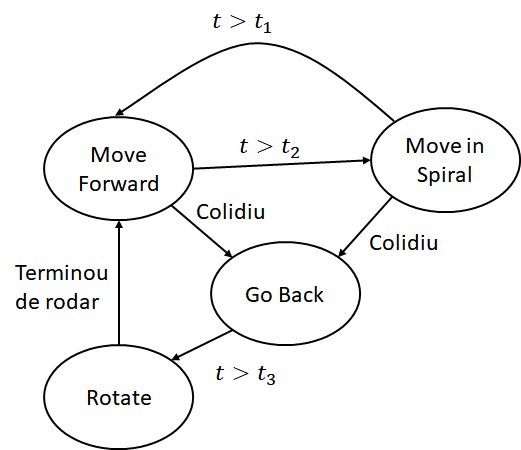
\includegraphics[width=0.4\textwidth]{FSM} % caminho até a figura "teste.png"
	\caption{Máquina de estados finita do robô Roomba.} % legenda da figura
	\label{fig:FSM}  % label da figura. ex: \label{fig:test}
\end{figure} 

Somente o arquivo \verb|state_machine.py| foi alterado, no qual as classes \verb|MoveForwardState|, \verb|MoveInSpiralState|, \verb|GoBackState| e \verb|RotateState| foram alteradas para realizar a operação esperada.

Para contabilizar o tempo, foi criada uma variável cotadora de número de chamadas do \texttt{behavior.update(agent)} chamada \texttt{number\_calls} para cada classe de estado. A cada chamada do método \texttt{execute} de um estado, a respectiva variável é incrementada de 1.

\subsubsection{\texttt{class MoveForwardState(State)}}
Como o código principal começa com este estado, a variável contadora de chamadas foi inicializada em 0 no método \texttt{\_\_init\_\_} deste estado.

O método \texttt{check\_transition(agent, state\_machine)} contém a verificação do tempo de execução do estado e da colisão com a parede. A verificação do tempo é realizada comparando o número de chamadas do respectivo estado com o valor obtido pela multiplicação da frequência de amostragem pelo tempo definido na rotina \texttt{constants.py}: se é maior ou igual, muda para o estado \texttt{MoveInSpiralState()}. A verificação de colisão é realizada através do método do agente \texttt{get\_bumper\_state()}: se há colisão, muda para o estado \texttt{GoBackState()}.

O método \texttt{execute(agent)} incrementa a variável contadora de chamadas e configura o robô para andar em linha reta setando a velocidade linear para o valor \texttt{FORWARD\_SPEED} e a velocidade angular para 0, através do método \texttt{set\_velocity(linear\_velocity, angular\_velocity)} do agente.

\subsubsection{\texttt{class MoveInSpiralState(State)}}
De forma semelhante à anterior, a variável contadora de chamadas foi inicializada em 0 no método \texttt{\_\_init\_\_} deste estado e uma variável chamada \texttt{spiral\_radius}, representando o raio da espiral num dado momento, foi inicializada pelo valor constante \texttt{INITIAL\_RADIUS\_SPIRAL}.

O método \texttt{check\_transition(agent, state\_machine)} contém a verificação do tempo de execução do estado e da colisão com a parede. A verificação do tempo é realizada de forma semelhante ao \texttt{MoveForwardState()}: se é maior ou igual, muda para o estado \texttt{MoveForwardState()}. A verificação de colisão é realizada da mesma forma do \texttt{MoveForwardState()}.

O método \texttt{execute(agent)} incrementa a variável contadora de chamadas; incrementa o raio da espiral através da multiplicação do fator de crescimento \texttt{SPIRAL\_FACTOR} pelo \texttt{SAMPLE\_TIME}; e configura o robô para andar em espiral setando a velocidade linear para o valor \texttt{FORWARD\_SPEED} e a velocidade angular para \texttt{FORWARD\_SPEED / spiral\_radius} (velocidade angular em curva de raio \texttt{spiral\_radius} considerando movimento circular uniforme), através do método \texttt{set\_veloci ty(linear\_velocity, angular\_velocity)} do agente.

\subsubsection{\texttt{class GoBackState(State)}}
Esta classe tem comportamento semelhando à \texttt{MoveForwardState()}, com a diferença de usar a velocidade \texttt{BACKWARD\_SPEED} no método \texttt{execute(agent)}, comparar com o tempo definido para andar para trás e mudar para o estado \texttt{RotateState()}. Esta classe não verifica colisão.

\subsubsection{\texttt{class RotateState(State)}}
Além de inicializar o contador de chamadas, o método \texttt{\_\_init\_\_} desta classe também escolhe um ângulo aleatória e uniformemente no intervalo $[-\pi,\pi)$, o qual será o ângulo de rotação em torno do eixo do robô.

O método \texttt{check\_transition(agent, state\_machine)} verifica se o robô já rotacionou todo o ângulo escolhido inicialmente e ao término muda para o estado \texttt{MoveForwardState()}.

Além de incrementar o contador de chamadas, o método \texttt{execute(agent)} seta a velocidade angular do robô para que ele rotacione ao redor do seu eixo, com velocidade positiva se o ângulo escolhido é positivo e vice-versa.

\subsection{\textit{Behavior Tree}}
%% Sugestão: cerca de meia página.
A Figura \ref{fig:BT} mostra um diagrama de blocos representando a\textit{behavior tree} utilizada neste projeto.

\begin{figure}[H]
	\centering
	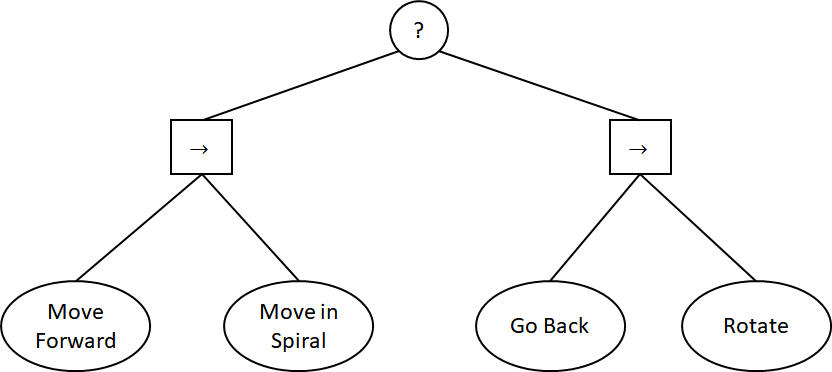
\includegraphics[width=0.6\textwidth]{BT} % caminho até a figura "teste.png"
	\caption{\textit{Behavior tree} de comportamento do robô Roomba.} % legenda da figura
	\label{fig:BT}  % label da figura. ex: \label{fig:test}
\end{figure} 

Somente o arquivo \verb|behavior_tree.py| foi alterado, no qual as classes \verb|RoombaBehaviorTree|, \verb|MoveForwardNode|, \verb|MoveInSpiralNode|, \verb|GoBackNode| e \verb|RotateNode| foram alteradas para realizar a operação esperada.

A contagem de chamadas foi efetuada de forma semelhante à máquina de estados finita, mas, neste caso, toda vez que a raiz da árvore era chamada e em cada nó da árvore.

O que foi feito nos métodos \texttt{\_\_init\_\_} dos estados da máquina de estados finita foi feito nos métodos \texttt{enter(agent)} das folhas da árvore. Nenhum código foi escrito nos métodos \texttt{\_\_init\_\_} das classes das folhas da árvore.

O método \texttt{execute(agent)} das folhas \texttt{GoBackNode} e \texttt{RotateNode} não retornam \texttt{FAILURE} dado que não verificam a colisão com as paredes. Por outro lado, o das outras duas folhas retornam \texttt{FAILURE} quando há colisão.

O funcionamento macro das folhas é semelhante aos estados da máquina de estados finita. A diferença é que, enquanto o tempo de execução não é alcançado, o método \texttt{execute(agent)} das folhas vão retornar \texttt{RUNNING}. E quando o tempo de execução finaliza, ele vai retornar \texttt{SUCCESS}.

\subsubsection{\texttt{class RoombaBehaviorTree(BehaviorTree)}}
O método \texttt{\_\_init\_\_} desta classe foi implementada de forma a criar a árvore de comportamentos para o robô Roomba. A raiz da árvore é um nó do tipo \textit{Selector}. Depois se atribui um filho a esta raiz, o qual é do tipo \textit{Sequence}. A este filho se atribui como filhos as folhas \verb|MoveForwardNode| e \verb|MoveInSpiralNode|, nesta ordem.

Depois se adiciona outro filho do tipo \textit{Sequence} à raiz da árvore. A este filho se atribui como filhos as folhas \verb|GoBackNode| e \verb|RotateNode|, nesta ordem.

\section{Figuras Comprovando Funcionamento do Código}

\subsection{Máquina de Estados Finita}
%% Basta colocar as figuras
\begin{figure}[H]
	\centering
	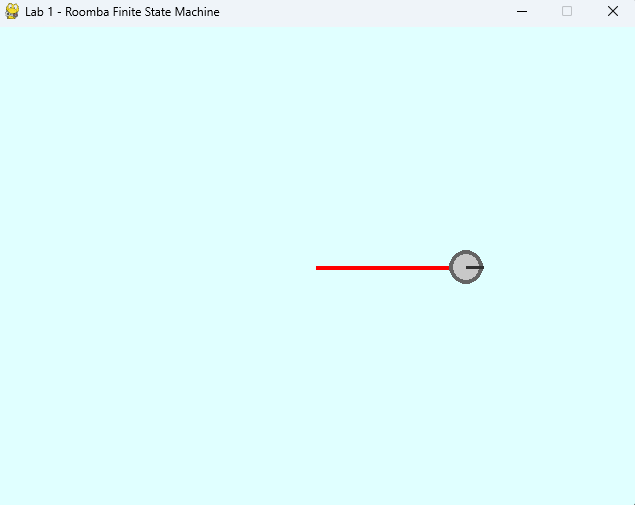
\includegraphics[width=0.5\textwidth]{FSM_forward} % caminho até a figura "teste.png"
	\caption{Máquina de estados finita: movendo em frente.} % legenda da figura
	\label{fig:FSM_forward}  % label da figura. ex: \label{fig:test}
\end{figure}

\begin{figure}[H]
	\centering
	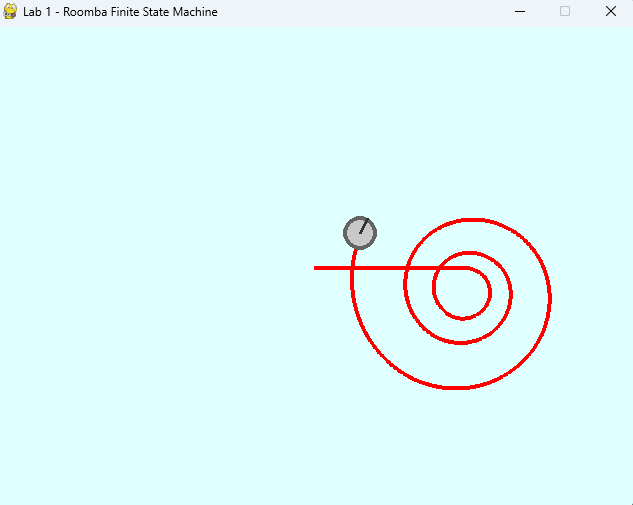
\includegraphics[width=0.5\textwidth]{FSM_spiral} % caminho até a figura "teste.png"
	\caption{Máquina de estados finita: movendo em espiral.} % legenda da figura
	\label{fig:FSM_spiral}  % label da figura. ex: \label{fig:test}
\end{figure}

\begin{figure}[H]
	\centering
	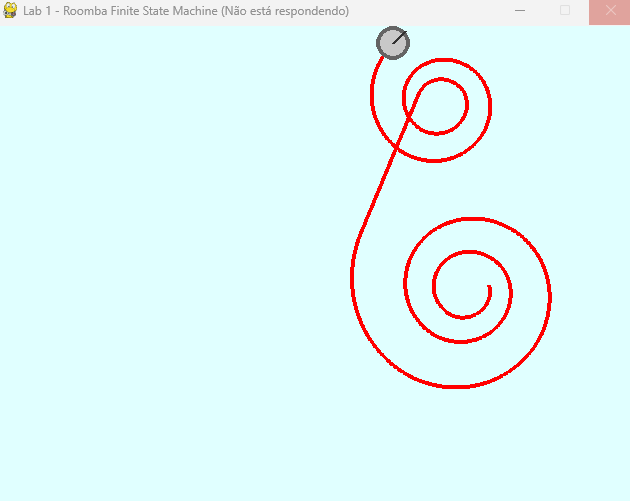
\includegraphics[width=0.5\textwidth]{FSM_collide} % caminho até a figura "teste.png"
	\caption{Máquina de estados finita: colidindo com a parede.} % legenda da figura
	\label{fig:FSM_collide}  % label da figura. ex: \label{fig:test}
\end{figure}

\begin{figure}[H]
	\centering
	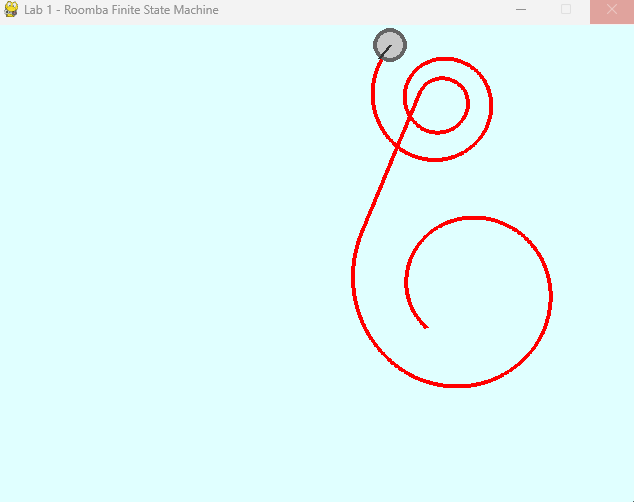
\includegraphics[width=0.5\textwidth]{FSM_back_rotate} % caminho até a figura "teste.png"
	\caption{Máquina de estados finita: rotacionando depois de vir para trás.} % legenda da figura
	\label{fig:FSM_back_rotate}  % label da figura. ex: \label{fig:test}
\end{figure}

\begin{figure}[H]
	\centering
	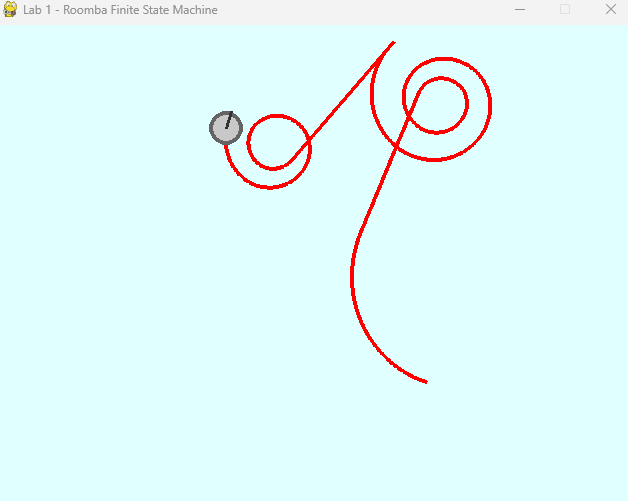
\includegraphics[width=0.5\textwidth]{FSM_continue} % caminho até a figura "teste.png"
	\caption{Máquina de estados finita: continuando depois de rotacionar.} % legenda da figura
	\label{fig:FSM_continue}  % label da figura. ex: \label{fig:test}
\end{figure}

\subsection{\textit{Behavior Tree}}
%% Basta colocar as figuras
\begin{figure}[H]
	\centering
	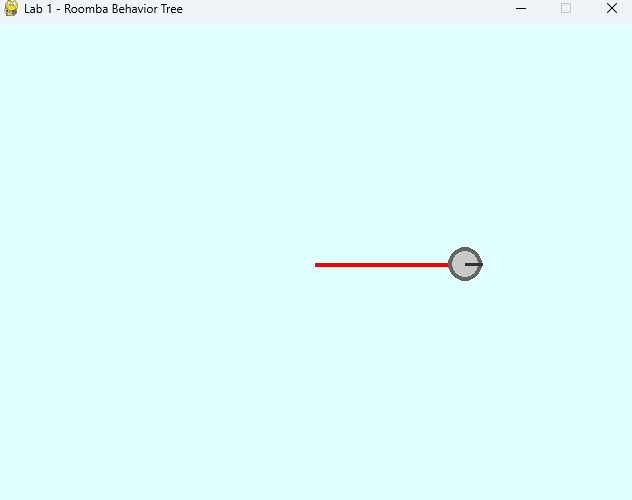
\includegraphics[width=0.5\textwidth]{BT_forward} % caminho até a figura "teste.png"
	\caption{Máquina de estados finita: movendo em frente.} % legenda da figura
	\label{fig:BT_forward}  % label da figura. ex: \label{fig:test}
\end{figure}

\begin{figure}[H]
	\centering
	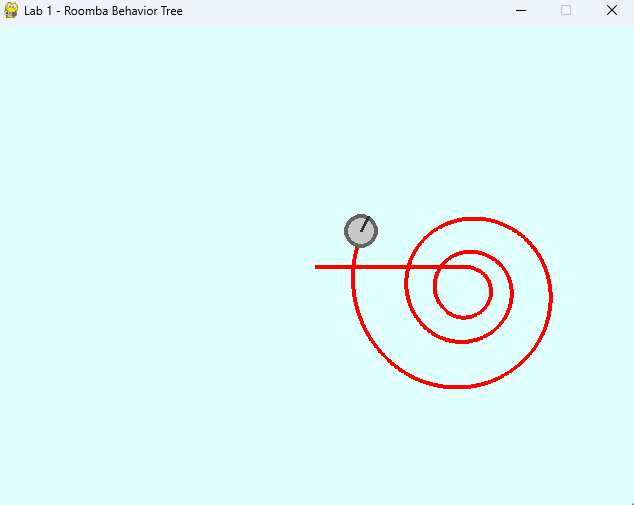
\includegraphics[width=0.5\textwidth]{BT_spiral} % caminho até a figura "teste.png"
	\caption{Máquina de estados finita: movendo em espiral.} % legenda da figura
	\label{fig:BT_spiral}  % label da figura. ex: \label{fig:test}
\end{figure}

\begin{figure}[H]
	\centering
	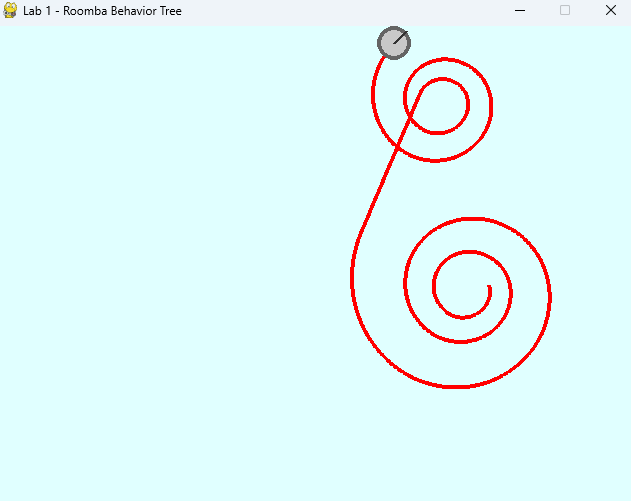
\includegraphics[width=0.5\textwidth]{BT_collide} % caminho até a figura "teste.png"
	\caption{Máquina de estados finita: colidindo com a parede.} % legenda da figura
	\label{fig:BT_collide}  % label da figura. ex: \label{fig:test}
\end{figure}

\begin{figure}[H]
	\centering
	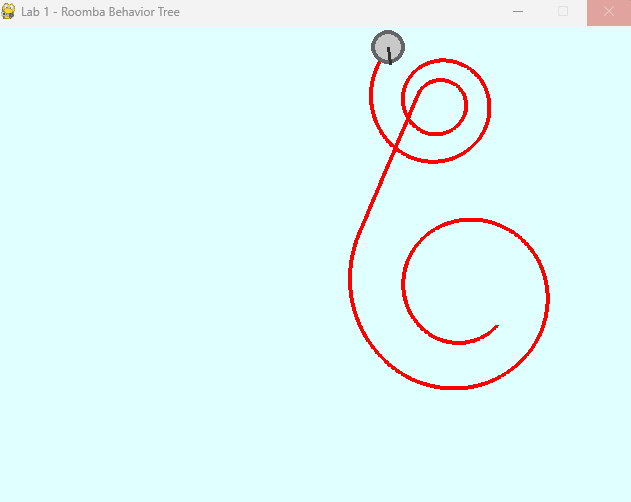
\includegraphics[width=0.5\textwidth]{BT_back_rotate} % caminho até a figura "teste.png"
	\caption{Máquina de estados finita: rotacionando depois de vir para trás.} % legenda da figura
	\label{fig:BT_back_rotate}  % label da figura. ex: \label{fig:test}
\end{figure}

\begin{figure}[H]
	\centering
	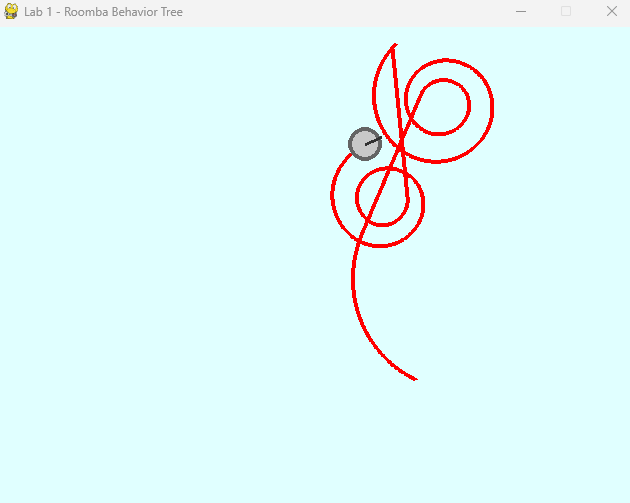
\includegraphics[width=0.5\textwidth]{BT_continue} % caminho até a figura "teste.png"
	\caption{Máquina de estados finita: continuando depois de rotacionar.} % legenda da figura
	\label{fig:BT_continue}  % label da figura. ex: \label{fig:test}
\end{figure}

\end{document}


%-----------------------------------------------------------------------------------------------
%       SUGESTÃO PARA ADICIONAR A FIGURA
%-----------------------------------------------------------------------------------------------
%
% \begin{figure}[H]
% \centering
% \includegraphics[width=0.7\textwidth]{teste.png} % caminho até a figura "teste.png"
% \caption{escreva aqui a legenda da figura} % legenda da figura
% \label{<label da figura>}  % label da figura. ex: \label{fig:test}
% \end{figure}  


%-----------------------------------------------------------------------------------------------
%       REFERENCIAR FIGURA NO TEXTO
%-----------------------------------------------------------------------------------------------
% \ref{<label da figura>}       
%
% Por ex: na Figura \ref{fig:test}, observa-se que...


%-----------------------------------------------------------------------------------------------
%       COPIAR LINHAS DE CÓDIGO EM TEXTO
%-----------------------------------------------------------------------------------------------
%
% \begin{minted}{python}
%     def print_hello_world():
%         '''
%         This function prints "Hello World!"
%         '''
%         print("Hello World!")
        
%     print_hello_world()
% \end{minted}
%
%-----------------------------------------------------------------------------------------------